```tex
\section{Verity Framework}

The Verity credibility graph is an information model based on the network structure consisting of sources and claims. Let us define it as:

\[
G = (S, C, E)
\]

where \(S\) is the set of sources, \(C\) is the set of claims, and \(E\) is the set of assertions which link sources to the claims they assert. This approach allows us to represent the information distribution across independent publishers as a graph. We use this graph as the foundation for credibility inference throughout the framework.

\subsection{Sources}

A source refers to an individual publisher that asserts one or more claims. Examples of sources may include websites, organizations, and databases. Every source is mapped to a unique node in the credibility graph.

\subsection{Claims}

A claim refers to a piece of information about an underlying entity. The same claim may be asserted by multiple different sources. Whereas other sources may assert conflicting claims about that same entity. Claims form nodes that connect different sources within the credibility graph.

\subsection{Assertions}

Assertions refer to the relationship that exists between a source and a claim. Whenever a source makes a claim, an assertion is created which connects the corresponding source node to the claim node. Assertions are what form the overall graph structure, revealing the distribution of claims amongst several sources.

\subsection{Credibility Graph}

The credibility graph is made up of two types of nodes - sources and claims. The assertions link these node types to form a bipartite graph where sources can only connect with claims and claims can only connect with sources. Figure~\ref{fig:credibility-graph} illustrates a simplified example of the graph.

\begin{figure}[ht]
    \centering
    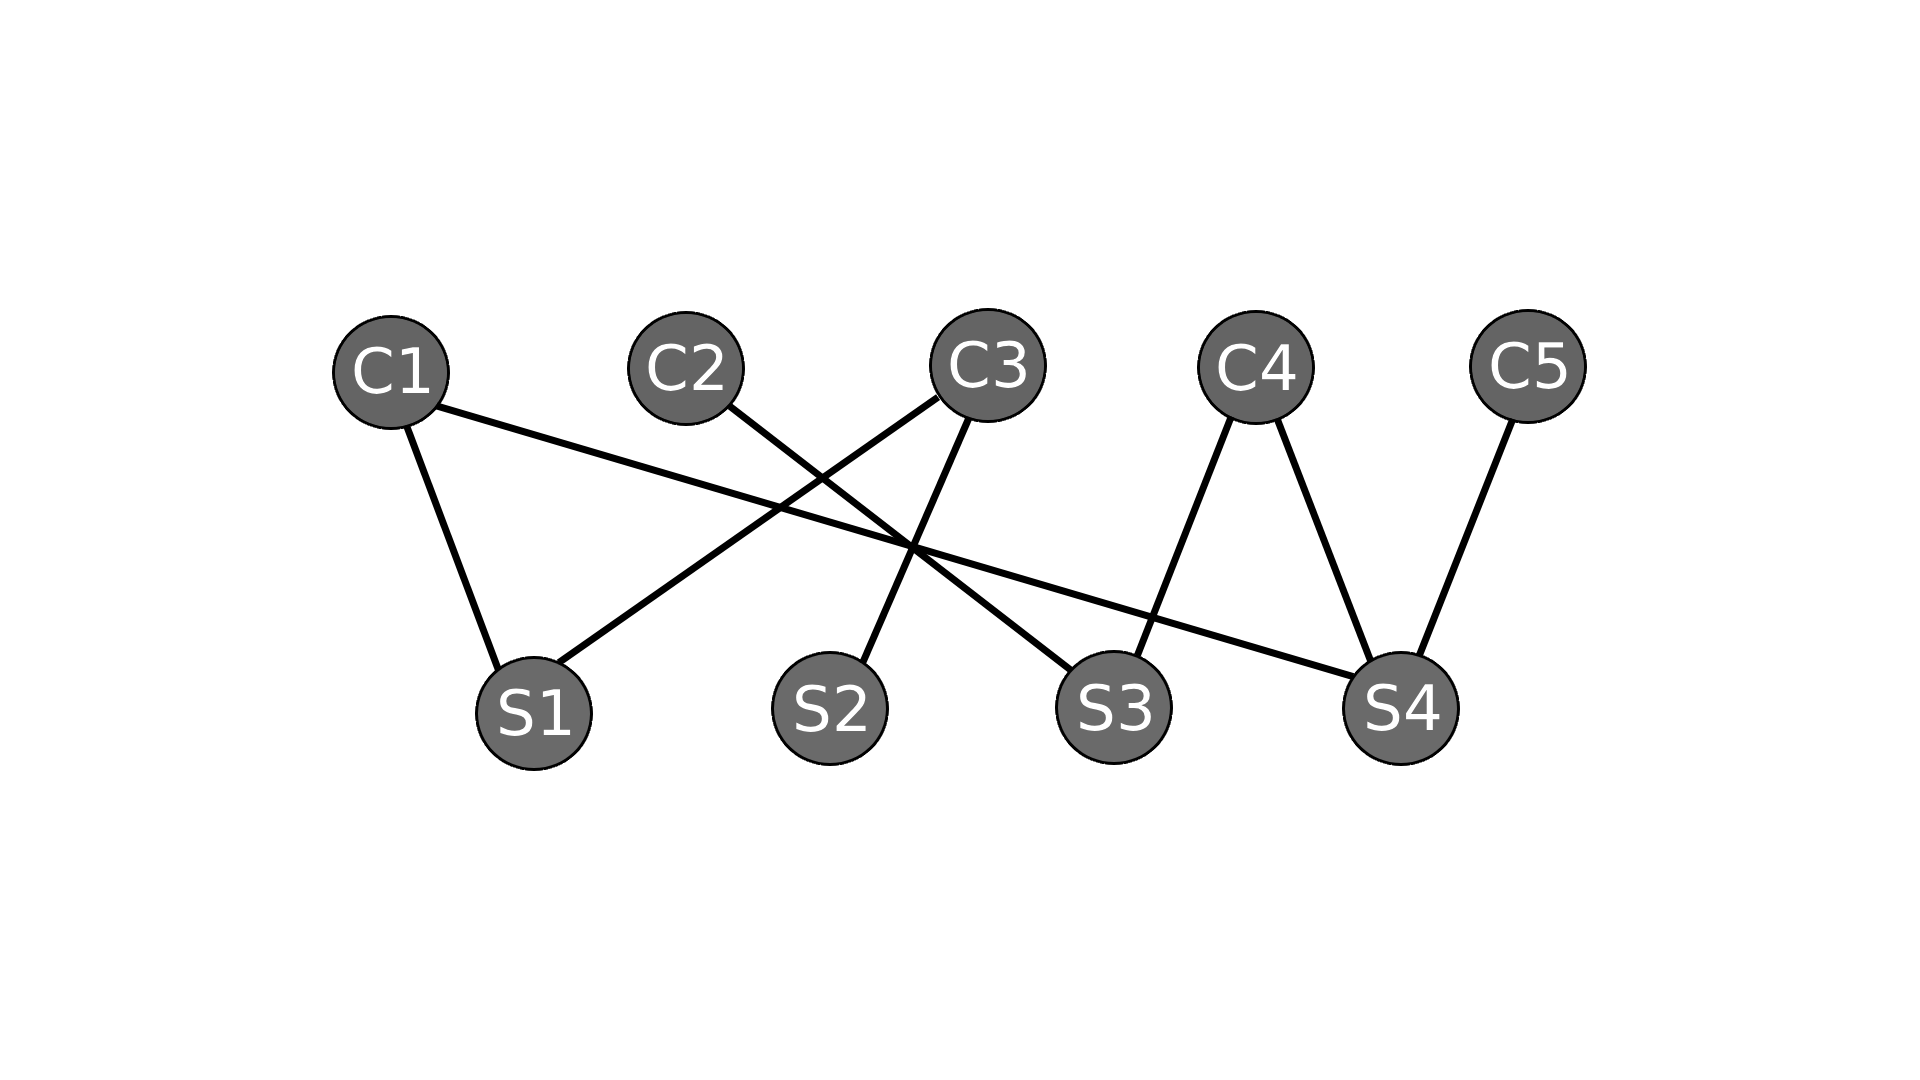
\includegraphics[width=0.8\textwidth]{figures/credibility_graph.png}
    \caption{Source nodes (bottom) connect to the claim nodes (top) they assert. Each edge indicates one assertion.}
    \label{fig:credibility-graph}
\end{figure}
```
